\chapter{Parallelization using MPI}

Throughout this chapter we will discuss how our serial implementation was parallelized. The parallelization was done
using MPI, and we will be referring to concept found in this library whenever relevant.

\section{Model for Communication}

We would like to share the work onto multiple processors, to parallelize our serial implementation. Looking at our
implementation it seems obvious to give each processor a set of cells to be responsible for, instead of giving each
processor a set of particles to be responsible for. By letting each processor be responsible for a zone, it can
perform most of the work completely locally, since each cell can only contain particles that will be affected by
particles in neighboring zones. This means that only particles lying in a cell at the border of the zone, may be
affected by a cell not owned by the local processor.

There are several ways in which the grid may be divided into zones for the processors. For the sake of simplicity
each processor is given some number of rows in the grid, for which they are responsible. This means that any processor
will have at most two neighboring processors, the one responsible for the rows above, and the one for the rows below.

\begin{figure}[H]
  \centering
  \begin{minipage}[b]{0.9\textwidth}
    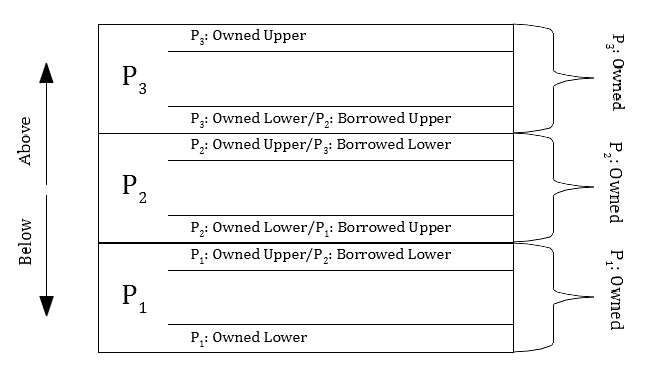
\includegraphics[width=\textwidth]{zones.png}
    \caption{Splitting the grid into zones.}
  \end{minipage}
  \label{fig:zones}
\end{figure}

% TODO Wording

To deal with the problems of the zones lying at the border of a zone, we've introduced the concept of borrowed and owned
zones as shown in figure \ref{fig:zones}. These zones are exactly correspond to exactly one row in the grid. Each
processor will contain up-to-date ``borrowed'' copies of these zones. The figure how each processor identifies the
different zones. Each processor will have to communicate with its neighbors to keep these zones in sync.

\section{Initializing the System}

The initial system is initialized at the root. Once all the particles have been created, a local grid is created, like
in the serial version. This gives us the initial distribution, which is then distributed to all the processors in the
system using \verb!MPI_Scatterv!.

\section{Synchronization of Nodes}

As discussed previously, each processor will need to keep synchronized copies of zones that they borrow
from each other. Since we in every iteration may make a change to these zones, we will need to perform this
synchronization step in every single iteration as well. The synchronization process is two-fold, first we gather up-to-
date information, and then we merge our information to get a correct picture of the system.

\textbf{Step 1: Synchronize Processors}

At the beginning of every iteration, we will need to synchronize all processors, such that they are all ready for the
next iteration. Once they are ready for the next iteration, we may begin exchanging information. This synchronization
can be done using the \verb!MPI_Barrier! procedure.

\textbf{Step 2: Prepare for Exchange with Neighbors}

A processors' neighboring processes will expect a complete image of how the zone it is borrowing looks. This message 
needs to be prepared, such that we can transmit it, this process consists solely of packing all the particle into a 
single buffer.

Before beginning the exchange, we will also clear out any particles that reside inside of the borrowed zones. This is
done since we will receive a completely new zone from our neighbors.

\textbf{Step 3: Exchange Message with Neighbors}

Once the messages are ready, we may exchange data with our neighbors. For efficiency reasons we use \verb!MPI_SendRecv!,
which allows for simultaneously sending and receiving data between two nodes. MPI requires that both parties involved in
the transfer, call this function with each other as arguments. For this reason, the following pattern has been
established: processors with an even rank communicate with the processor above it first, while processors with an odd
rank will communicate with the processor below first. The exchange process between two processors go like this:

\begin{enumerate}
	\item Exchange sizes (in particles) of zones
	\item Exchange the particles, this exchange requires the knowledge of how many particles we will receive
	\item Exchange sizes of local insertions into borrowed zones
	\item Exchange particles involved in local insertions into borrowed zones
\end{enumerate}

It should also be noted that this means that the synchronization process for the system as a whole, will only take the
time of communicating with each neighbor, since these are all done in parallel.

\textbf{Step 4: Update the World}

We have already discussed that we share our owned zones with our neighbors. The reason for this fairly simple, we're the
ones responsible for updating these zones, hence we are the ones capable of telling our neighbors about updates made in
it.

However, it is also possible for particles to migrate from one processor to another. Hence we need to track whenever we
perform an insertions of particles from our owned zone into a borrowed zone. These particles are all tracked in a
separate buffer, and exchanged with the neighbor in step 3.

The insertions that we receive from our neighbors are then merged together with our own local view to give a completely
up-to-date view of the system.

\textbf{Step 5: Cleanup}

Finally we clear out our local insertions from an owned zone into a borrowed zone. Such that we're ready for the next 
iteration.

\section{Running the Simulation and Combining the Result}

The simulation step itself is left mostly unchanged from the original serial implementation. It should however be noted
that we only have to directly look at the particles we own ourselves. That is we do not need to loop directly over the
particles in the borrowed zones, since if any of our owned particles collide with them, then this will be picked up when
we look at the neighboring cells.

While the simulation is running, we write down where are particles are. To be able to merge the particles later, we have
had to add an ID number to every particle, such that we may track any particle, even if it goes through several
processors. Once the simulation is done, it is collected at the root node using \verb!MPI_Gatherv!, sorted per
iteration, and ID, and saved to the output file.

\section{Limitations}

The technique used for distributing the cells to each processor, puts some limitations to the number of processors one
can effectively use with the system. The current implementation allows for at most as many processors as there are rows.
And when hitting this case, we won't be very effective, since we will hold twice as many borrowed cells, that we hold
owned cells. The system could allow for more processors by letting the zones be smaller squares, that do not need to
have the same width as the entire grid. This does however come at the cost of having up to four neighbors instead of at
most two.

\section{Performance}
\begin{enumerate}
  \item Overall performance 
  \item Breakdown of time used in a single run
\end{enumerate}

\section{Testing}
\begin{enumerate}
  \item{(Should also be added to serial)}
  \item Testing stuff
\end{enumerate}